\section{欧姆定律}\label{sec:8-7}

第五节的实验告诉我们,导体中的电流强度跟这段导体两端的电压成正比。

第六节关于电阻的学习又告诉我们,在电压不变的情况下,导体的电阻越大,通过导体的电流越小。
进一步研究第五节中的两次实验记录还会发现电阻跟电流的定量关系。

例如,在电压是 2 伏特的情况下,

电阻是 5 欧姆的导线 $AB$ 中的电流是 0.4 安培,

电阻是 10 欧姆的导线 $CD$ 中的电流是 0.2 安培。

又例如,在电压是 4 伏特的情况下,

电阻是 5 欧姆的导线 $AB$ 中的电流是 0.8 安培,

电阻是 10 欧姆的导线 $CD$ 中的电流是 0.4 安培。

如果 $CD$ 的电阻不是 $AB$ 的两倍,而是三倍或四倍,那么 $CD$ 中的电流就是 $AB$ 中的三分之一或四分之一。

可见,在电压一定的情况下,导体中的电流强度跟导体的电阻成反比。

综合起来,我们可以得到下面的结论:
\textbf{导体中的电流强度,跟这段导体两端的电压成正比,跟这段导体的电阻成反比}。

这个结论是德国物理学家欧姆在十九世纪初期研究电压和电流强度的关系的基础上得出的,通常就叫做\textbf{欧姆定律}。

如果用 $U$ 表示导体两端的电压,$R$ 表示导体的电阻,$I$ 表示导体中的电流强度,那么,欧姆定律可以写成
$$ I = \dfrac{U}{R} \;\juhao $$
式中的 $I$、$U$、$R$ 的单位分别为安培、伏特、欧姆。

欧姆定律在实际工作中有很重要的应用。利用欧姆定律,我们不但可以计算出通过导体的电流强度,
还可以计算出让用电器正常工作需加多大的电压,以及测定导体的电阻。
下面让我们举几个实例来说明这些应用。

\begin{enhancedline}
\liti 并联的红、绿、白三盏电灯,它们两端的电压都是 220 伏特,电阻分别是 3230 欧姆、1210 欧姆、484 欧姆,求通过各盏电灯的电流强度。

通过各灯的电流强度,根据欧姆定律 $I = \dfrac{U}{R}$ 是容易计算的。但是应用欧姆定律公式时必须明确:
\CJKunderwave*{欧姆定律公式中的 $I$、$U$、$R$ 是同一段电路上的电流强度、电压、电阻}。
要计算通过红灯的电流强度,只能用红灯的电阻去除红灯两端的电压,而不能甩绿灯或白灯的电阻去除。
为了便于我们分析问题,最好先根据题意画个电路图,在图上注明已知量的符号、数值和各未知量的符号(图 \ref{fig:8-17})。

\begin{wrapfigure}[7]{r}{8cm}
    \centering
    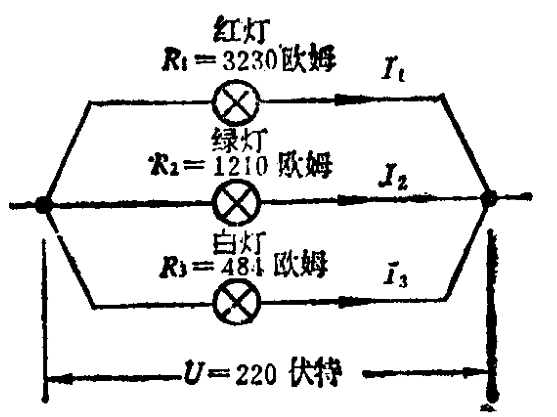
\includegraphics[width=7.5cm]{../pic/czwl2-ch8-17}
    \caption{}\label{fig:8-17}
\end{wrapfigure}
\jie $\begin{aligned}[t]
    I_1 & = \dfrac{U}{R_1} = \dfrac{220\fute}{3230\oumu} \approx 0.07 \anpei\;\juhao \\
    I_2 & = \dfrac{U}{R_2} = \dfrac{220\fute}{1210\oumu} \approx 0.18 \anpei\;\juhao \\
    I_3 & = \dfrac{U}{R_3} = \dfrac{220\fute}{484\oumu}  \approx 0.45 \anpei\;\juhao
\end{aligned}$

答:通过红灯、绿灯、白灯的电流强度分别是 0.07 安培, 0.18 安培, 0.45 安培。


\liti 一个小灯泡,正常发光时应该通过 0.6 安培的电流,电阻是 6.3 欧姆。
要使它正常发光,需要在小灯泡两端加多大的电压?

在这道题中,已经知道小灯泡的电阻 $R$ 和应该通过的电流强度 $I$,只要把欧姆定律公式 $I = \dfrac{U}{R}$
变形为 $U = IR$,就可以求出小灯泡两端需要加的电压 $U$。

解:$U = IR = 0.6\anpei \times 6.3\oumu \approx 3.8\fute$。

答:需要在小灯泡两端加 3.8 伏特的电压。


\liti 用伏特表测出电路中某导体两端的电压是 6 伏特,用安培表测出这个导体中的电流强度是 0.2 安培。求这个导体的电阻。

解: 从欧姆定律公式 $I = \dfrac{U}{R}$, 可以得到:

\hspace{3em}$R = \dfrac{U}{I} = \dfrac{6\fute}{0.2\anpei} = 30\oumu$。

答:这个导体的电阻是 30 欧姆。
\end{enhancedline}

从例题 3 可以知道,如果分别用伏特表和安培表测出电路中某一导体上的电压和导体中的电流强度,
就可以根欧坶定律算出这个导体的电阻。因此,欧姆定律给我们提供了一种常用的测定电阻的方法;
这种用伏特表、安培表测电阻的方法通常叫做伏安法。


\section*{阅读材料}

\begin{wrapfigure}[12]{r}{6cm}
    \centering
    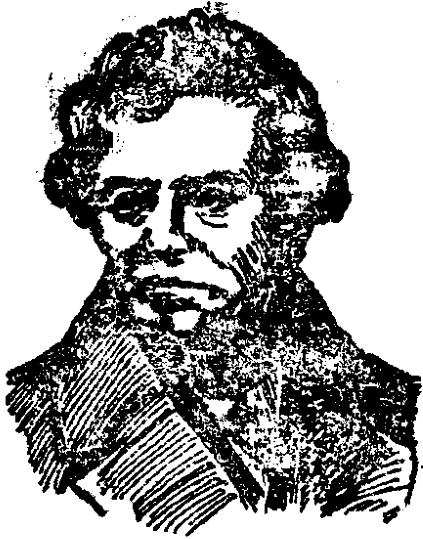
\includegraphics[width=5cm]{../pic/czwl2-ch8-ohm}
    \caption*{欧姆(1787 ~ 1854)}\label{fig:8-ohm}
\end{wrapfigure}

欧姆对电流定律的研究,主要是在 1817 到 1827 年他担任中学物理教师期间进行的。
现在我们看欧姆定律的公式那么简单。但是,在当时欧姆为了研究这一问题,付出了十年的心血。
那时的实验条件很差,没有现成的仪器可用。他当时能得到的电压稳定的电源,只能提供几毫伏的电压,
灵敏的测电流的仪器和各种电阻值的导体,都要靠他自己动手制备。
他能够完成这些精细的制作和精确的实验,都得利于年青时在他父亲的制锁作坊里练出的一双巧手。


\lianxi

(1) 车床照明灯采用 36 伏特的安全工作电压。如果车床照明灯工作时的灯丝电阻是 32 欧姆,这时通过灯丝的电流强度是多大?

(2) 安培表的电阻是很小的,某安培表的电阻是 0.02 欧姆,允许通过的最强电流是 3 安培,
超过 3 安培,表会受到损伤,甚至被烧坏。
这个安培表能直接连在电压是 2 伏特的蓄电池的两极上吗?

(3) 电子手表的电源是一个小钮扣似的氧化银电池。电子手表的电阻大约是多少欧姆?

(4) 有一个电烙铁,工作时电阻丝里的电流强度是 0.5 安培,如果电阻是 72 欧姆,电烙铁两端的电压是多少伏特?

(5) 电路里串联着一个 3 欧姆的定值电阻和一个安培表,安培表的示数是 1.2 安培。
能不能用量程是 3 伏特的伏特表,来测量定值电阻上的电压?

(6) 你知道你家里电灯两端的电压是多大吗?
如果灯泡正常发光时通过的电流强度是 0.2 安培,这时灯泡的电阻是多少欧姆?

(7) 一段导体两端电压是 2 伏特时,导体中的电流强度是 0.5 安培。
如果两端的电压增大到 4 伏特,导体中的电流强度是多大?
如果电压减小到 1 伏特,电流强度又是多大?

(8) 一个定值电阻两端的电压是 3 伏特时,它的电流强度是 0.5 安培。
如果电压是 5 伏特时,能不能用量程是 0.6 安培的安培表来测量这个定值电阻里的电流强度?

